\let\negmedspace\undefined
\let\negthickspace\undefined
\documentclass[journal]{IEEEtran}
\usepackage[a5paper, margin=10mm, onecolumn]{geometry}
%\usepackage{lmodern} % Ensure lmodern is loaded for pdflatex
\usepackage{tfrupee} % Include tfrupee package

\setlength{\headheight}{1cm} % Set the height of the header box
\setlength{\headsep}{0mm}     % Set the distance between the header box and the top of the text

\usepackage{gvv-book}
\usepackage{gvv}
\usepackage{cite}
\usepackage{amsmath,amssymb,amsfonts,amsthm}
\usepackage{algorithmic}
\usepackage{graphicx}
\usepackage{textcomp}
\usepackage{xcolor}
\usepackage{txfonts}
\usepackage{listings}
\usepackage{enumitem}
\usepackage{mathtools}
\usepackage{gensymb}
\usepackage{comment}
\usepackage[breaklinks=true]{hyperref}
\usepackage{tkz-euclide} 
\usepackage{listings}
% \usepackage{gvv}                                        
\def\inputGnumericTable{}                                 
\usepackage[latin1]{inputenc}                                
\usepackage{color}                                            
\usepackage{array}                                            
\usepackage{longtable}                                       
\usepackage{calc}                                             
\usepackage{multirow}                                         
\usepackage{hhline}                                           
\usepackage{ifthen}                                           
\usepackage{lscape}
\usepackage{circuitikz}
\tikzstyle{block} = [rectangle, draw, fill=blue!20, 
    text width=4em, text centered, rounded corners, minimum height=3em]
\tikzstyle{sum} = [draw, fill=blue!10, circle, minimum size=1cm, node distance=1.5cm]
\tikzstyle{input} = [coordinate]
\tikzstyle{output} = [coordinate]


\begin{document}

\bibliographystyle{IEEEtran}
\vspace{3cm}

\title{4.8.35}
\author{AI25BTECH11039-Harichandana Varanasi}
 \maketitle
% \newpage
% \bigskip
{\let\newpage\relax\maketitle}

\renewcommand{\thefigure}{\theenumi}
\renewcommand{\thetable}{\theenumi}
\setlength{\intextsep}{10pt} % Space between text and floats


\numberwithin{equation}{enumi}
\numberwithin{figure}{enumi}
\renewcommand{\thetable}{\theenumi}



\date{}

\begin{document}
\maketitle




\noindent\textbf{Question.} \;
$y=10^{x}$ is the reflection of $y=\log_{10}x$ in the line whose equation is \underline{\hspace{3cm}}.

\bigskip
\noindent\textbf{Solution.}
\begingroup
\setcounter{equation}{0}
\renewcommand{\theequation}{\arabic{equation}}

Let the mirror line be written in normal form
\begin{equation}
  \vec{n}^{\top}\vec{x}=c,                                   \label{eqL}
\end{equation}
with normal $\vec{n}\in\mathbb{R}^{2}$ and variable vector $\vec{x}\in\mathbb{R}^{2}$.


A point on the curve $y=\log_{10}u$ is
\begin{equation}
    \vec{Q}(t)=\myvec{t\\ \log_{10}t}, \qquad t>0 .
\end{equation}


Its reflection in the line \eqref{eqL} is 
\begin{equation}
  \vec{R}(t)=\vec{Q}(t)-\frac{2\big(\vec{n}^{\top}\vec{Q}(t)-c\big)}{\|\vec{n}\|^{2}}\;\vec{n}. \label{eqR}
\end{equation}
For the image curve to be  $y=10^{x}$ we require
\begin{equation}
  \vec{R}(t)=\myvec{\log_{10}t\\ t}\quad \text{for all } t>0 . \label{eqTarget}
\end{equation}

Equating components in \eqref{eqR}--\eqref{eqTarget} and collecting the
independent functions $t$ and $\log_{10}t$ yields

\begin{equation}
  a^{2}=b^{2}, \qquad a\,b=-a\,b, \qquad c=0 .
\end{equation}
Hence $a=-b\neq 0$ and $c=0$.  Thus $\vec{n}\propto\myvec{1\\ -1}$ and the mirror line is
\begin{equation}
  \myvec{1 & -1}\vec{x}=0.                                   \label{eqAns}
\end{equation}

Therefore, the required line of reflection is
\[
  \boxed{\ \myvec{1\;\; -1}\vec{x}=0\ }\quad (\text{scalar form } y=x).
\]
\endgroup





\begin{figure}[H]
    \centering
    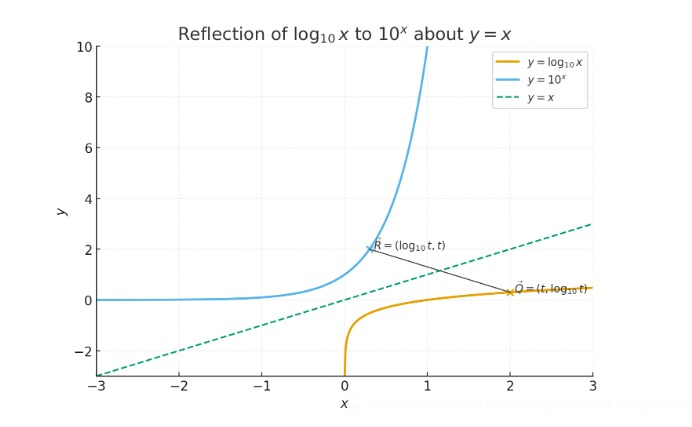
\includegraphics[width=0.8\linewidth]{figs/matgeo-4.13.4.jpeg}
    \caption{$y=\log_{10}x$ and $y=10^{x}$ with mirror line $y=x$.}
    \label{fig:4.13.4}
\end{figure}




 

\end{document}
